\section{Results}\label{chapterResults}

% Demographic information:
% Range of age, Geschlechterverteilung, Previous experience?
\subsection{Demographics}
We had 14 participants, 6 of them were male, 8 female. 
Their age was ranging from 24 to 34 years old and 5 people had corrected eye sight.
When asked about previous experiences in Virtual 
Reality 10 people out of 14 said they had little to no experience with it.
And 7 out of 14 people said they had little to no experience with video games prior to the experiment.
%When asked about their prior experience with VR on a scale of 0 to 6 the participants responded with an average of $2.53$.
%The average response for the question how much experience participants had with computer games prior to the experiment was $3.4$.

\subsection{Deviations \& Placement Accuracy}
We evaluated the participants' performances in terms of deviation of the placed object positions/rotations with regard to the respective target positions/rotations (i.e. position/rotation of the corresponding translucent shapes).
Positional deviation was recorded for each of the three coordinates $x$, $y$, and $z$ separately.
Likewise rotational deviation was recorded in degrees around all three axes $x$, $y$, and $z$ separately. %\textit{forward($x$)}, \textit{up($y$)}, and \textit{right($z$)} separately.

For each condition Table \ref{table:positional_deviation} lists the median \textit{positional} deviations of object placements after normalization across all participants.
The normalization was calculated as follows.
First, for each participant the positional deviations of their object placements were averaged.
The participants' resulting \textit{mean deviations} were then each divided by the largest mean deviation of all participants under the respective condition.
This ratio results in a \textit{normalized positional deviation} for each participant which becomes 0 when the participant positioned all their objects perfectly at the target positions.
It becomes 1 when the participant's mean deviation is the largest of all participants.
Finally the median of these values was then determined for each condition which is reported in the table \ref{table:positional_deviation}.
The same procedure was used to normalize the mean rotational deviations and subsequently calculate rotational accuracy, whose distributions could then be used to compare rotational accuracy between conditions (see figure \ref{fig:accuracy_rot_boxplot}) and is explained in more detail later on in this section.

Due to the varying symmetries of the different object groups \textit{rotational} deviations are evaluated separately for each of them.
E.g. rotating a cube by an integer multiple of $90^{\circ}$ around the \textit{up} axis results in the same relative orientation with regards to the target orientation.
For a 5-pointed star on the other hand the same relative orientation can be reached when rotating the object by a multiple of $72^{\circ}$ and for a 6-pointed star it is reached when rotating by a multiple of $60^{\circ}$.
Median rotational deviations for each object group are reported in tables
\ref{table:rotational_deviation_cubes}, \ref{table:rotational_deviation_5stars} and \ref{table:rotational_deviation_6stars} in degrees (i.e. without normalization).
Positional deviation is reported across all object types per condition.
This is because positional deviation was always calculated with respect to the center of the object and is therefore independent of object symmetries.

%In order to make the recordings from both conditions comparable to one another, the deviations were normalized to a value from 0 to 1.
%In this context a deviation of 0 designates the ideal placement of the object at its target position.
%A deviation of 1 on the other hand resembles the worst of all recorded placements for that particular object across participants.

%Rotational deviation was normalized for each object type separately.
%This was in order to account for the different object symmetries.

%Positional Deviation - figures/table
\begin{table}[htbp]
    \centering
    \begin{tabular}{|l|c c c|r|}
        \hline
        \textbf{Overall}	&	$dev_x$	&	$dev_y$	&	$dev_z$	\\ \hline
        Android	&	0.009	&	0.200	&	0.006	\\ \hline
        Leap	&	0.006	&	0.022	&	0.013	\\ \hline
    \end{tabular}
    \caption{
    \textsf{Median \textit{positional} deviations of object placements after normalization across all participants.}
    }
    \label{table:positional_deviation}
\end{table}

%Rotational Deviation - figures/table
%Cubes
\begin{table}[htbp]
    \centering
    \begin{tabular}{|l|c c c|}
        \hline
        \textbf{Cubes}	&	$dev_x$	&	$dev_y$	&	$dev_z$	\\ \hline
        Android	&	$0.15^{\circ}$	&	$0.10^{\circ}$	&	$1.45^{\circ}$	\\ \hline
        Leap	&	$0.75^{\circ}$	&	$1.4^{\circ}$	&	$13.15^{\circ}$	\\ \hline
    \end{tabular}
    \caption{
    \textsf{Median \textit{rotational} deviations in degrees between cube placements and their target orientations.}
    }
    \label{table:rotational_deviation_cubes}
\end{table}

%5-Pointed Stars
\begin{table}[htbp]
    \centering
    \begin{tabular}{|l|c c c|}	
        \hline 
        \textbf{5-Pointed Stars}	&	$dev_x$	&	$dev_y$	&	$dev_z$	\\ \hline
        Android	&	$0.00^{\circ}$	&	$0.30^{\circ}$	&	$1.35^{\circ}$	\\ \hline
        Leap	&	$4.25^{\circ}$	&	$4.55^{\circ}$	&	$11.05^{\circ}$	\\ \hline
    \end{tabular}
    \caption{
    \textsf{Median \textit{rotational} deviations in degrees between 5-pointed star placements and their target orientations.}
    }
    \label{table:rotational_deviation_5stars}
\end{table}

%6-Pointed Stars
\begin{table}[htbp]
    \centering
    \begin{tabular}{|l|c c c|}
        \hline
        \textbf{6-Pointed Stars}	&	$dev_x$	&	$dev_y$	&	$dev_z$	\\ \hline
        Android	&	$0.40^{\circ}$	&	$0.30^{\circ}$	&	$1.70^{\circ}$	\\ \hline
        Leap	&	$1.15^{\circ}$	&	$2.10^{\circ}$	&	$7.90^{\circ}$	\\ \hline
    \end{tabular}
    \caption{
    \textsf{Median \textit{rotational} deviations in degrees between 6-pointed star placements and their target orientations.}
    }
    \label{table:rotational_deviation_6stars}
\end{table}

 
To compare the quality of placement that could be achieved under each condition we compare the distribution of a \textit{rotational placement accuracy} $\alpha_{r}$ and \textit{positional placement accuracy} $\alpha_{p}$.
For calculating these accuracies we invert and then realign the respective normalized deviations to 1 as follows:
\begin{center}
$\alpha_{p} = 1-\overline{dev}_{p}$,
\end{center}
where $\overline{dev}_{p}$ is the medial normalized positional deviation within a particular group of objects and under a given condition.
And
\begin{center}
$\alpha_{r} = 1-\overline{dev}_{r}$,
\end{center}
where $\overline{dev}_{r}$ is the medial normalized rotational deviation within a particular group of objects and under a given condition.
The distribution of participant accuracies is reported in the form of box-plots in figures \ref{fig:accuracy_pos_boxplot} and \ref{fig:accuracy_rot_boxplot}.

% --- BOXPLOTTING: POSITOINAL ACCURACY
\begin{figure*}[htbp]
    \centering    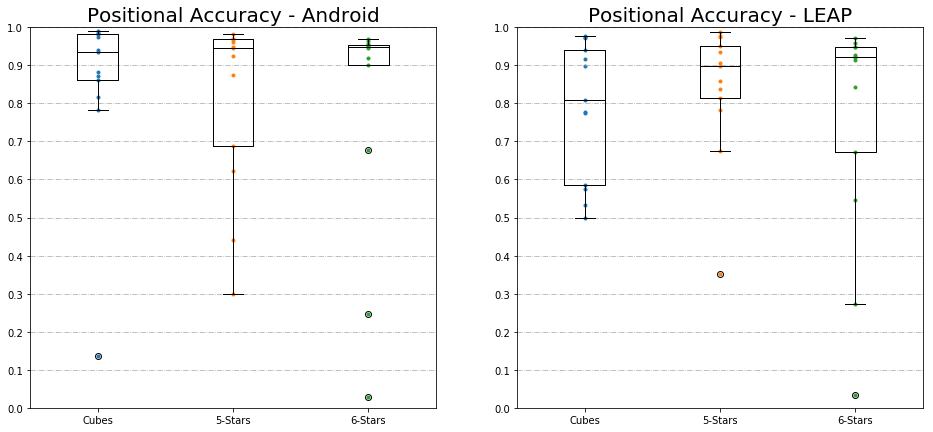
\includegraphics[width=1\textwidth]{figures/accuracy_pos_boxplot.png}
    \caption{
    \textsf{Distributions of positional placement-accuracies after normalization for different object groups in each condition.
    For calculating the placement accuracies the accuracies in each dimension $x$, $y$, $z$ have been averaged for each participant.
    The box extends from the lower (Q1) to the upper (Q3) quartile values of the data.
    Whiskers reach out to include data-points within 1.5 times the inter-quartile-range below/above the quartile Q1/Q3 respectively.
    Data-points outside the whiskers' reach may be considered outliers of the distribution.}
    }
    \label{fig:accuracy_pos_boxplot}
\end{figure*}
% --- BOXPLOTTING: ROTATIONAL ACCURACY
\begin{figure*}[htbp]
    \centering    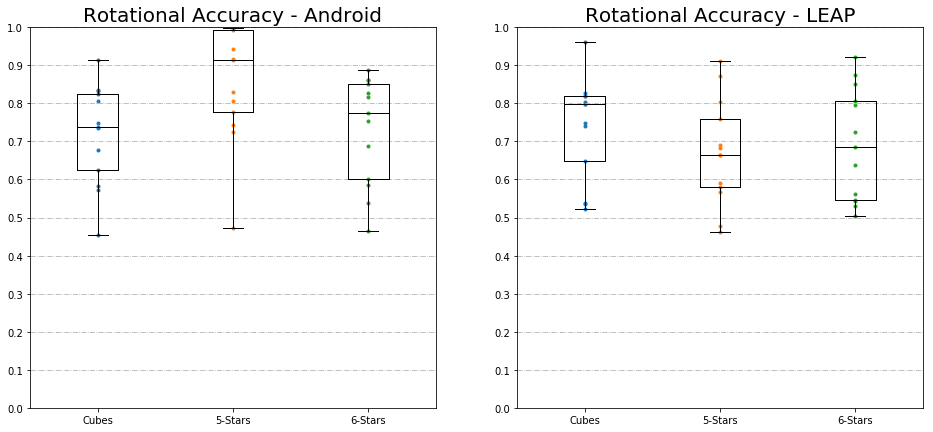
\includegraphics[width=1\textwidth]{figures/accuracy_rot_boxplot.png}
    \caption{
    \textsf{Distributions of rotational placement-accuracies after normalization for different object groups in each condition. For calculating the placement accuracies the accuracies in each dimension $x$, $y$, $z$ have been averaged for each participant.
    The box extends from the lower(Q1) to the upper(Q3) quartile values of the data.
    Whiskers reach out to include data-points within 1.5 times the inter-quartile-range below/above the quartile Q1/Q3 respectively.
    Data-points outside the whiskers' reach may be considered outliers of the distribution.}
    }
    \label{fig:accuracy_rot_boxplot}
\end{figure*}



\subsection{System Usability \& Task Workload}

% --- BARCHARTS: SUS & NASA-TLX
\begin{figure*}[htbp]
    \centering
   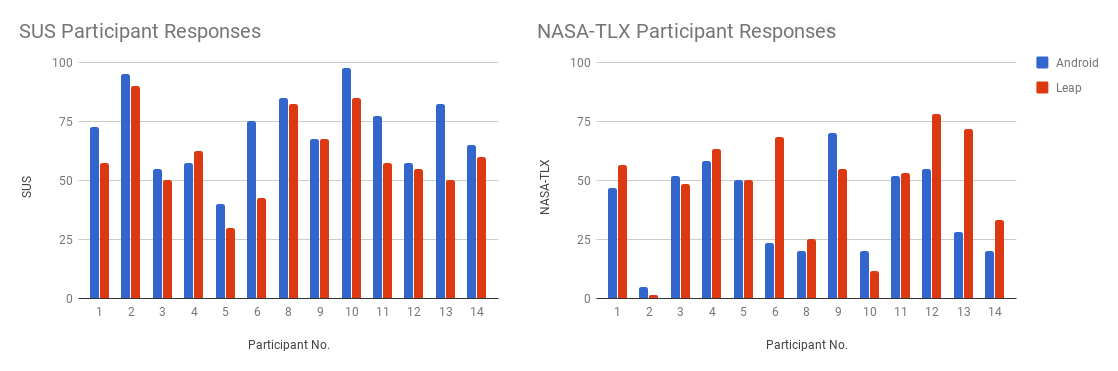
\includegraphics[width=1\textwidth]{figures/SUS_NASATLX_chart.png}
    \caption{
    \textsf{SUS and NASA-TLX responses as reported by participants after finishing the task under each condition. Average SUS across all participants was $61.83$ (LEAP) / $70.83$ (Android) (higher is better).
    Average NASA-TLX response was $46.89$ (LEAP) / $36.11$ (Android) (lower is better).}
    }
    \label{fig:sus_nasatlx_response}
\end{figure*}

% --- BOXPLOTTING: SUS & NASA-TLX ---
\begin{figure*}[htbp]
    \centering
    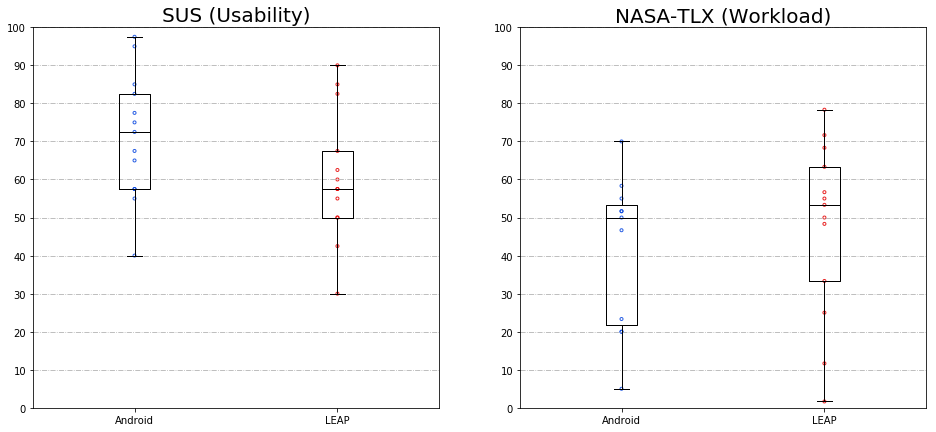
\includegraphics[width=1\textwidth]{figures/sus_nasatlx_boxplot.png}
    \caption{
    \textsf{Boxplots for SUS usability and NASA-TLX workload scores reported by all 15 participants after finishing the task under each condition.
    The box extends from the lower(Q1) to the upper(Q3) quartile values of the distribution.
    Whiskers reach out to include data-points within 1.5 times the inter-quartile-range below/above the quartile Q1/Q3 respectively.
    Data-points outside the whiskers' reach may be considered outliers of the distribution.}
    }
    \label{fig:sus_nasatlx_boxplots}
\end{figure*}

The \textit{System Usability Scale} (SUS) is a reliable tool for measuring the usability of an interactive system and yields a single number representing a composite measure.
It comprises of 10 questions; whose answers range from \textit{Strongly Agree} (5) to \textit{Strongly Disagree} (1).
Since it only has 5 answers, the scale is easy to administer to participants.
It also reliably relays if the condition is usable or unusable even for small sample sizes.
Interpreting the scoring on the other hand can be complex.
The participant’s scores for each question are converted to a new number, added together and then multiplied by 2.5 to convert the original scores from a scale of 0-40 to a scale from 0-100.
Still, these scores are not percentages and should be considered only in terms of their percentile ranking i.e. individual scores are not meaningful on their own.
This is to say that a system scoring a higher SUS may be considered more usable over another one, but it is not possible to quantify how much more usable it actually is from the difference in SUS alone.
To summarize the SUS score calculation:
\begin{itemize}
\item The scores from each of the questions are summed up.
\item For questions 1,3,5,7 and 9 the raw SUS score is the response - 1 (these questions are phrased positively and a higher response suggests a more easy-to-use system).
\item For questions 2,4,6,8 and 10, the raw SUS score is 5 minus the response (these questions are phrased negatively and a higher response suggests a more hard-to-use system).
\item Finally the sum of the scores (maximum 40 points) is multiplied by 2.5 to result in the SUS score (maximum 100 points).
\end{itemize}

Similar to SUS the \textit{NASA Task Load Index} combines a multitude of factors.
It provides an overall workload score which is based on a weighted average of ratings on six composite scales: 
\textit{Mental demands}, \textit{physical demands}, \textit{temporal demands}, \textit{own performance}, \textit{effort} and \textit{frustration}.
There exist procedures to determine a weighting based on the perceived importance of each factor from the participant's perspective.
For our study we used a linear weighting of each factor's contribution instead.
This was to save time during experiments which already took relatively long.
The score is determined by the response to six questions each with a possible response on a scale from 0-10.
Here a higher response suggests a higher workload experienced while performing the task.
A participant's responses are summed up and rescaled via dividing by 60 and multiplying with 100 to generate an index on a 0-100 scale.
\if false
The degree to which each of the six factors contribute to the workload of the specific task to be evaluated, from the raters' perspectives, is determined by their responses to pair-wise comparisons among the six factors.
Magnitude ratings on each subscale are obtained after each performance of a task or task segment. Ratings of factors deemed most important in creating the workload of a task are given more weight in computing the overall workload score, thereby enhancing the sensitivity of the scale.
\fi
Responses for SUS and NASA-TLX are reported in figure \ref{fig:sus_nasatlx_response} and their distributions across participants are visualized as box-plots in figure \ref{fig:sus_nasatlx_boxplots}.


\if false
%Workload and Usablity Scores - figures/table
\begin{table}[htbp]
    \centering
    \begin{tabular}{l|c c|c c}
    \toprule
    	{}	&	\multicolumn{2}{c}{SUS}	&	\multicolumn{2}{c}{NASA-TLX}\\
    \midrule
        {}	&	Android	&	LEAP	&	Android	& LEAP\\
        Average	&	$70.83$	& $61.83$	&	$46.89$	&	$36.11$\\
        SD	&	$16.76$	&	$16.30$	&	$20.86$	&	$22.87$\\
    \bottomrule
    \end{tabular}
    \caption{
    \textsf{---}
    }
    \label{table:sus_nasatlx}
\end{table}
\fi